\section*{Skæring mellem 2 linjer}

At beregne skæringen mellem 2 linjer er det samme som at løse 2 ligninger med 2 ubekendte. For at løse 2 ligninger med 2 ubekendte vil vi benytte os af erstatningsmetoden. Proceduren for erstatningsmetoden kan ses nedenfor

\begin{frm-thm}{Erstatningsmetoden}
\begin{enumerate}
\item Isoler x i den ene af de 2 ligninger
\item Indsæt det isolerede udtryk for x ind på x's plads i den anden ligning
\item Isoler y i den anden ligning
\item Indsæt den fundne værdi for y på y's plads i det isolerede udtryk for x
\end{enumerate}

\end{frm-thm}

\subsection*{Eksempel:}

Find skæringen mellem de 2 linjer givet ved forskrifterne

\begin{align*}
y = 2x - 4 && y = 5x + 2
\end{align*}

For at finde skæringen mellem de 2 linjer skal vi løse 2 ligninger med 2 ubekendte. Step 1 er at isolere x i den ene af ligningerne. Vi isolerer nu x i ligningen $y = 2x - 4$

\begin{align*}
&y = 2x - 4\\
\Updownarrow \hspace*{2mm} &\\
&y + 4 = 2x && \text{Flytter 4 over på den anden side}\\
\Updownarrow \hspace*{2mm} &\\
&\frac{y + 4}{2} = \frac{2x}{2} && \text{Dividerer med 2 på begge sider}\\
\Updownarrow \hspace*{2mm} &\\
&\frac{y + 4}{2} = x
\end{align*}

Vi har nu isoleret x i den ene ligning og er kommet frem til udtrykket $x = \frac{y + 4}{2}$.

Step 2 siger at vi skal indsætte det isolerede udtrkyk for x på x's plads i den anden ligning og step 3 at vi derefter skal isolere y. 

\begin{align*}
&y = 5x + 2 \\
\Updownarrow \hspace*{2mm} &\\
&y = 5\left(\frac{y + 4}{2}\right) + 2 && x = \frac{y + 4}{2}\\
\Updownarrow \hspace*{2mm} &\\
&y = \frac{5(y + 4)}{2} + 2 \\
\Updownarrow \hspace*{2mm} &\\
&y = \frac{5y + 20}{2} + 2 \\
\Updownarrow \hspace*{2mm} &\\
&y \cdot 2 = \frac{5y + 20}{2}\cdot 2 + 2 \cdot 2 && \text{Ganger med 2 på alle led for at få brøken til at forsvinde}\\
\Updownarrow \hspace*{2mm} &\\
&2y = 5y + 20 + 4 \\
\Updownarrow \hspace*{2mm} &\\
&2y - 5y = 24 && \text{Flytter de 5y over på den anden side}\\
\Updownarrow \hspace*{2mm} &\\
&-3y = 24 \\
\Updownarrow \hspace*{2mm} &\\
&\frac{-3y}{-3} = \frac{24}{-3} && \text{Dividerer med -3 for at isolere y}\\
\Updownarrow \hspace*{2mm} &\\
&y = -8
\end{align*}

Vi udførere nu step 4 som siger at vi skal indsætte den fundne værdi for y, $y = -8$ ind i det isolerede udtryk for x, $x = \frac{y + 4}{2}$.

\begin{align*}
&x = \frac{y + 4}{2}\\
\Updownarrow \hspace*{2mm} &\\
&x = \frac{-8 + 4}{2} && y = -8\\
\Updownarrow \hspace*{2mm} &\\
&x = \frac{-4}{2} = -2
\end{align*}

Da vi nu har fundet en værdi for både x og y, har vi netop fundet skæringen mellem de 2 linjer. Skæringen mellem de 2 linjer er $(x,y) = (-2, -8)$.

Vi viser nu hvordan man kan kontrollere sit resultat i GeoGebra.

\newpage

Først intaster man forskriften for de 2 linjer i input feltet som kan ses på figuren nedenfor

\begin{figure*}[ht]
    \centering
    \begin{subfigure}[t]{0.5\textwidth}
        \centering
        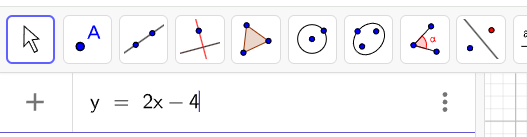
\includegraphics[width=0.5\textwidth]{img_1}
        \caption{Input feltet med funktionen $y = 2x-4$ indtastet}
    \end{subfigure}%
    ~ 
    \begin{subfigure}[t]{0.5\textwidth}
        \centering
        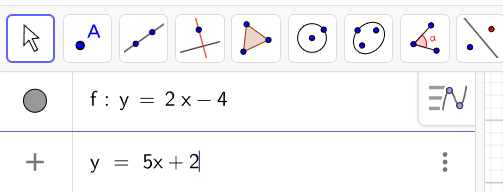
\includegraphics[width=0.5\textwidth]{img_2}
        \caption{Input feltet med funktionen $y = 5x+2$ indtastet}
    \end{subfigure}
    \caption{Indtastning af funktioner i input feltet i GeoGebra}
\end{figure*}


Derefter vælger man skæringsværktøjet og klikker på begge linjer. Et punkt vil dukke op der hvor linjerne skærer hinanden og vi kan aflæse punktets koordinater som kan ses på figuren nedenfor

\begin{figure*}[ht]
    \centering
    \begin{subfigure}[t]{0.5\textwidth}
        \centering
        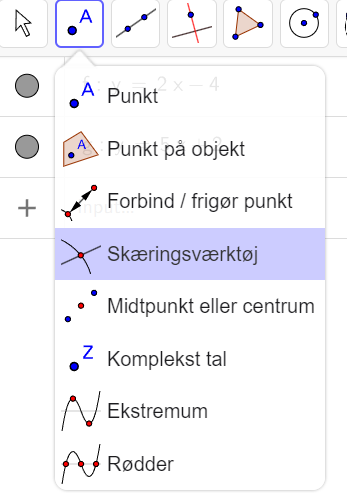
\includegraphics[width=0.5\textwidth]{img_3}
        \caption{Valg af skæringsværktøj}
    \end{subfigure}%
    ~ 
    \begin{subfigure}[t]{0.5\textwidth}
        \centering
        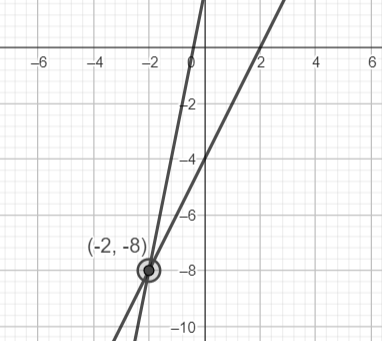
\includegraphics[width=0.5\textwidth]{img_4}
        \caption{Skæringspunktet mellem de 2 linjer}
    \end{subfigure}
    \caption{Kontrol af skæringspunktet mellem 2 linjer i GeoGebra}
\end{figure*}


Som vi kan se matcher skæringspunktet med skæringspunktet $(-2, -8)$ vi beregnede os til.








\subsection*{Opgaver}


\textbf{Opgave 1:}

Bestem skæringen mellem de 2 linjer med forskrifterne 

\begin{align*}
y = 5x - 4 &&  y = x + 4
\end{align*}

\textbf{Opgave 2:}

Bestem skæringen mellem de 2 linjer med forskrifterne 

\begin{align*}
y =  5x-8 &&  y = -4x + 10
\end{align*}

\textbf{Opgave 3:}

Bestem skæringen mellem de 2 linjer med forskrifterne 

\begin{align*}
y = 2x + 2 &&  y = -2x + 2
\end{align*}

\textbf{Opgave 4:}

Bestem skæringen mellem de 2 linjer med forskrifterne 

\begin{align*}
y = 2x + 10 &&  y = -2x - 6
\end{align*}

\textbf{Opgave 5:}

Bestem skæringen mellem de 2 linjer med forskrifterne 

\begin{align*}
y = 2x - 4 &&  y = -2x -12
\end{align*}

\textbf{Opgave 6:}

Bestem skæringen mellem de 2 linjer med forskrifterne 

\begin{align*}
y = -4x +10 &&  y = 3x -11
\end{align*}

\textbf{Opgave 7:}

Bestem skæringen mellem de 2 linjer med forskrifterne 

\begin{align*}
y = -4x +10 &&  y = -2x -2
\end{align*}

\textbf{Opgave 8:}

Bestem skæringen mellem de 2 linjer med forskrifterne 

\begin{align*}
y = -2x +10 &&  y = 4x -2
\end{align*}

\textbf{Opgave 9:}

Bestem skæringen mellem de 2 linjer med forskrifterne 

\begin{align*}
y = 3x +12 &&  y = -4x -2
\end{align*}

\textbf{Opgave 10:}

Bestem skæringen mellem de 2 linjer med forskrifterne 

\begin{align*}
y = 3x +12 &&  y = -4x -30
\end{align*}


\newpage


\subsection*{Facit}


\textbf{Opgave 1:}

\begin{figure}[ht]
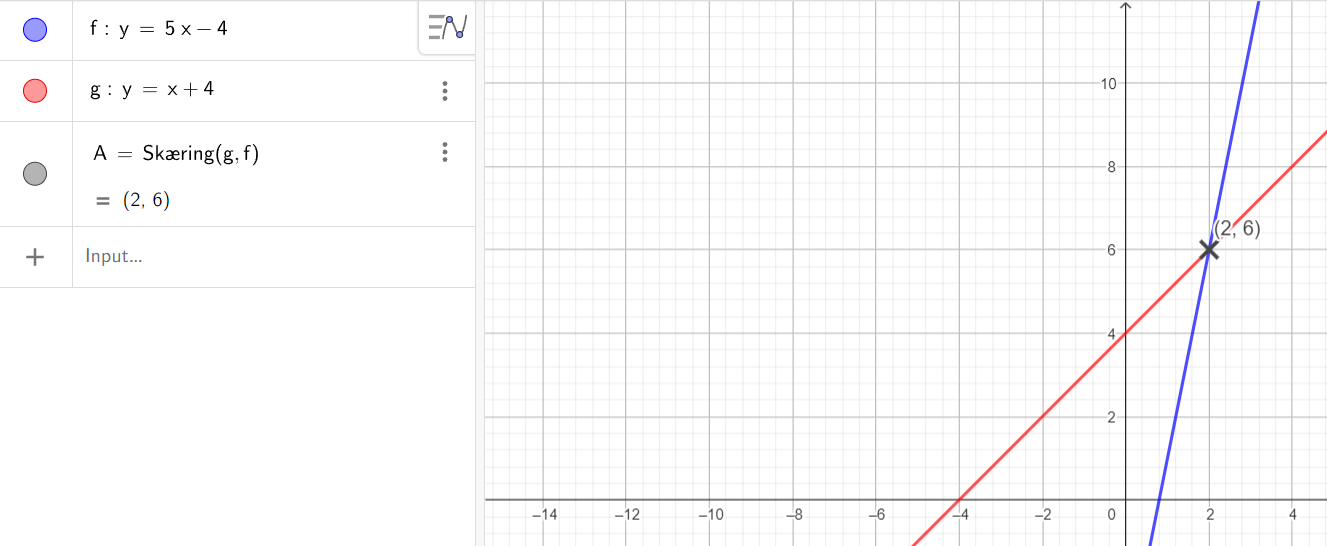
\includegraphics[width=0.8\textwidth, height=0.25\textwidth]{ans_1}
\caption{Skæringspunktet $(2,6)$ mellem de 2 linjer $y = 5x - 4$ og $y = x + 4$}
\end{figure}

\textbf{Opgave 2:}

\begin{figure}[ht]
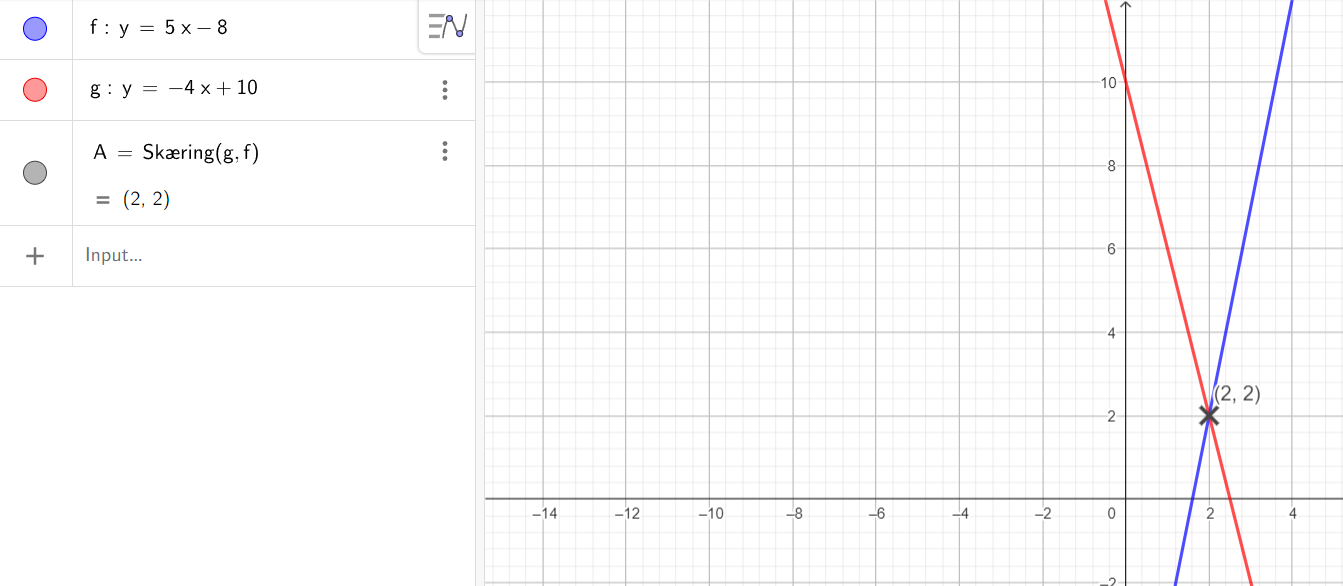
\includegraphics[width=0.8\textwidth, height=0.25\textwidth]{ans_2}
\caption{Skæringspunktet $(2,2)$ mellem de 2 linjer $y = 5x - 8$ og $y = -4x + 10$}
\end{figure}

\textbf{Opgave 3:}

\begin{figure}[ht]
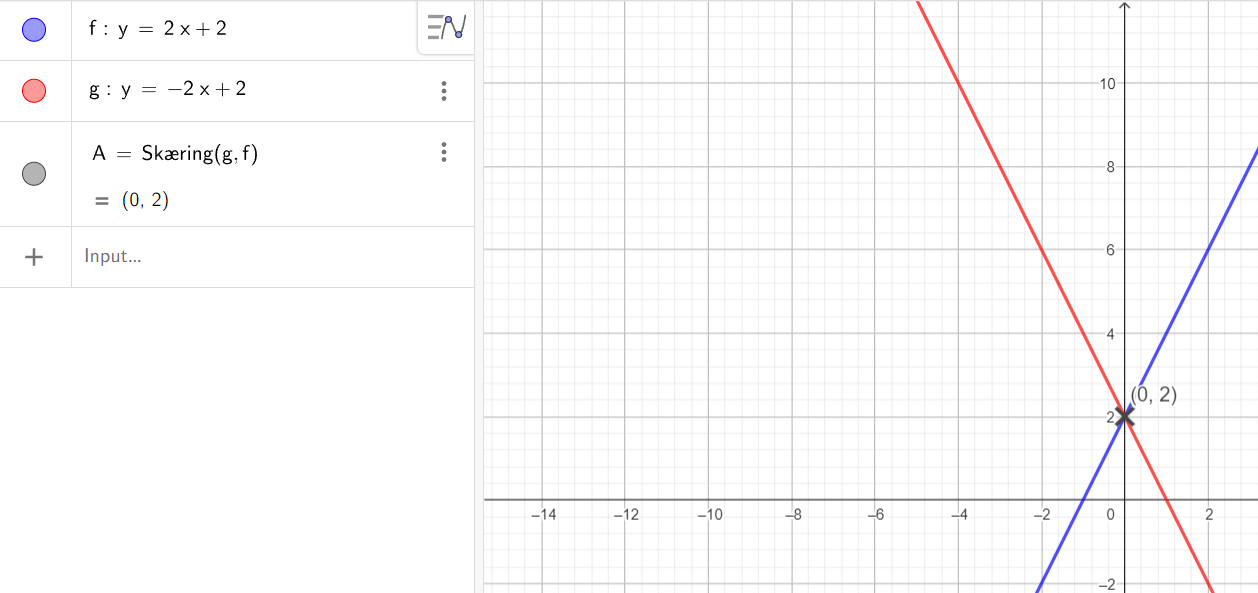
\includegraphics[width=0.8\textwidth, height=0.25\textwidth]{ans_3}
\caption{Skæringspunktet $(0,2)$ mellem de 2 linjer $y = 2x + 2$ og $y = -2x + 2$}
\end{figure}

\newpage

\textbf{Opgave 4:}

\begin{figure}[ht]
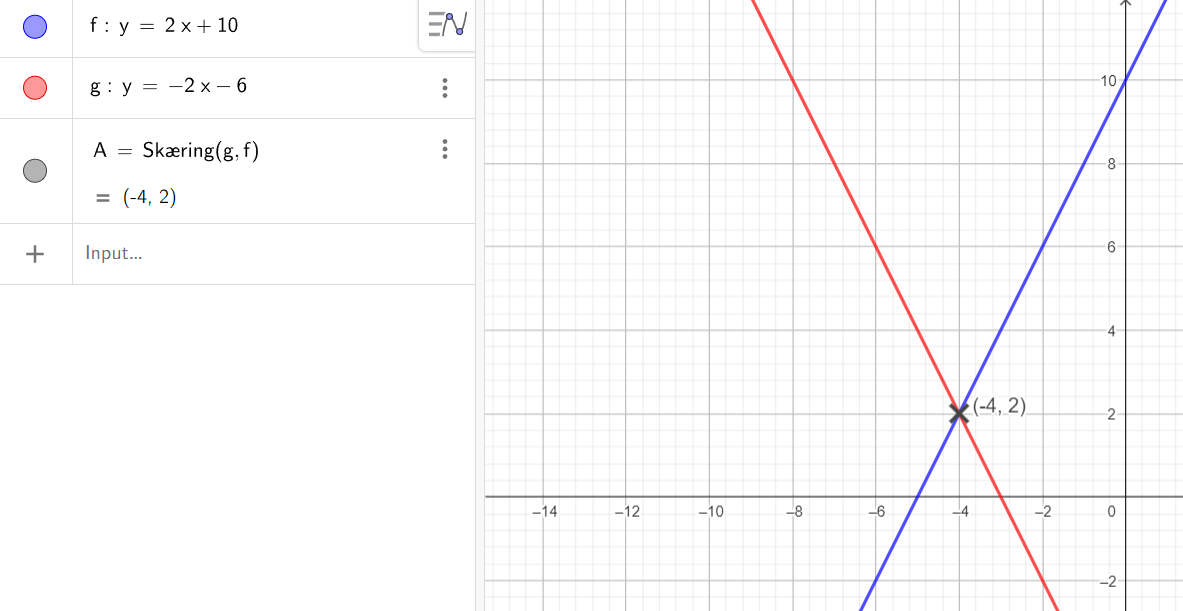
\includegraphics[width=0.8\textwidth, height=0.25\textwidth]{ans_4}
\caption{Skæringspunktet $(-4,2)$ mellem de 2 linjer $y = 2x + 10$ og $y = -2x -6$}
\end{figure}

\textbf{Opgave 5:}

\begin{figure}[ht]
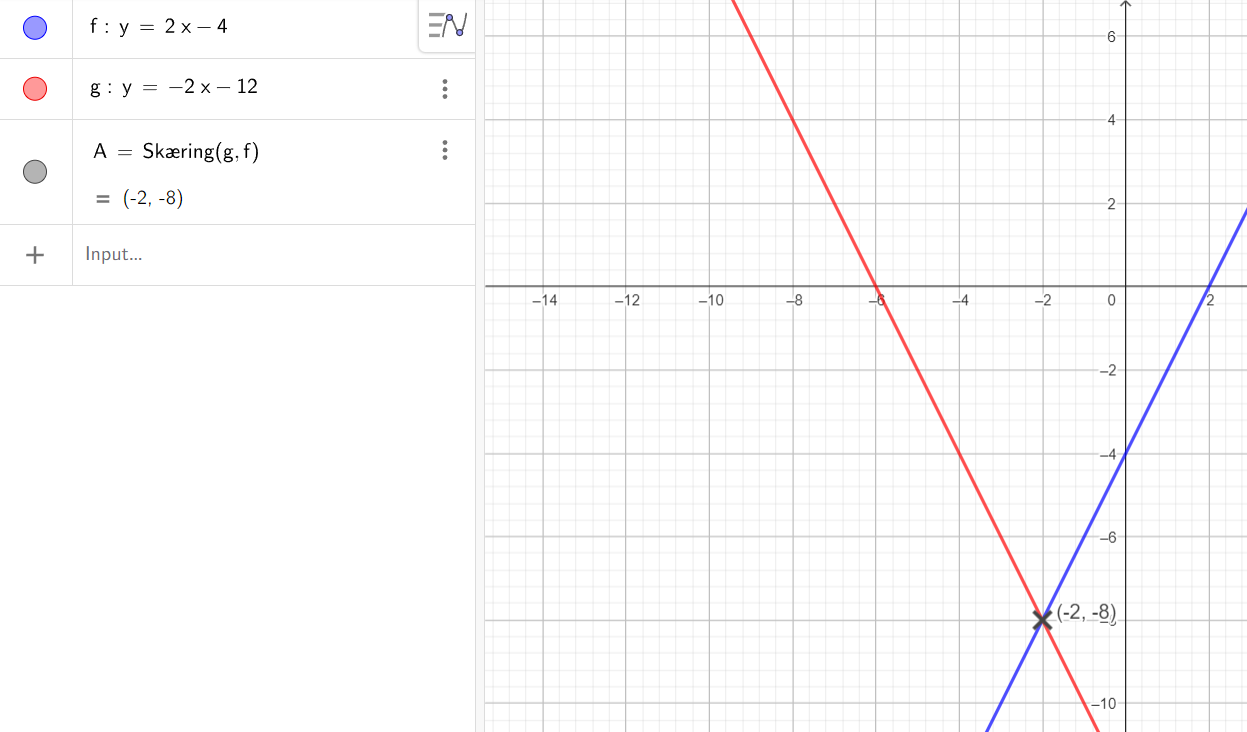
\includegraphics[width=0.8\textwidth, height=0.25\textwidth]{ans_5}
\caption{Skæringspunktet $(-2,-8)$ mellem de 2 linjer $y = 2x - 4$ og $y = -2x -12$}
\end{figure}

\textbf{Opgave 6:}

\begin{figure}[ht]
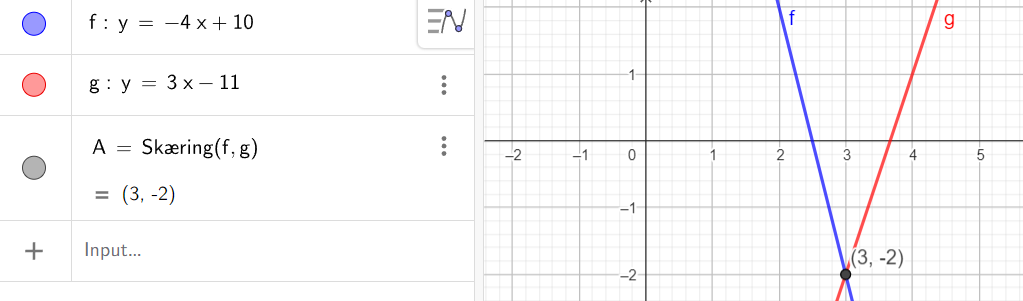
\includegraphics[width=0.8\textwidth, height=0.25\textwidth]{ans_6}
\caption{Skæringspunktet $(3,-2)$ mellem de 2 linjer $y = -4x + 10$ og $y = 3x -11$}
\end{figure}

\newpage

\textbf{Opgave 7:}

\begin{figure}[ht]
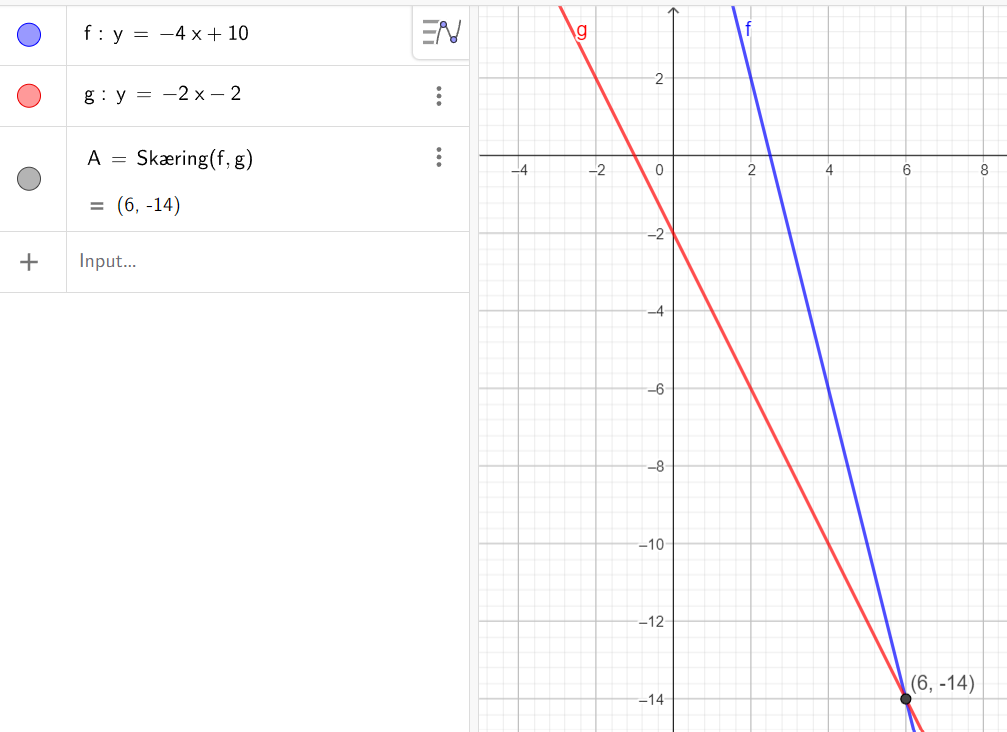
\includegraphics[width=0.8\textwidth, height=0.26\textwidth]{ans_7}
\caption{Skæringspunktet $(6,-14)$ mellem de 2 linjer $y =-4x + 10$ og $y = -2x -2$}
\end{figure}

\textbf{Opgave 8:}

\begin{figure}[ht]
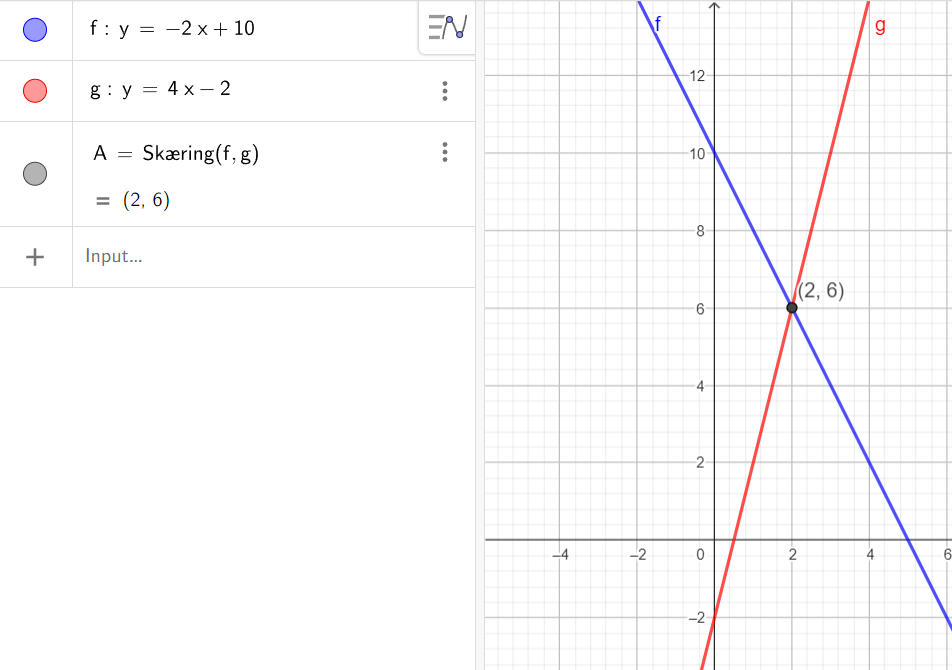
\includegraphics[width=0.8\textwidth, height=0.26\textwidth]{ans_8}
\caption{Skæringspunktet $(2,6)$ mellem de 2 linjer $y = -2x +10$ og $y = 4x -2$}
\end{figure}

\textbf{Opgave 9:}

\begin{figure}[ht]
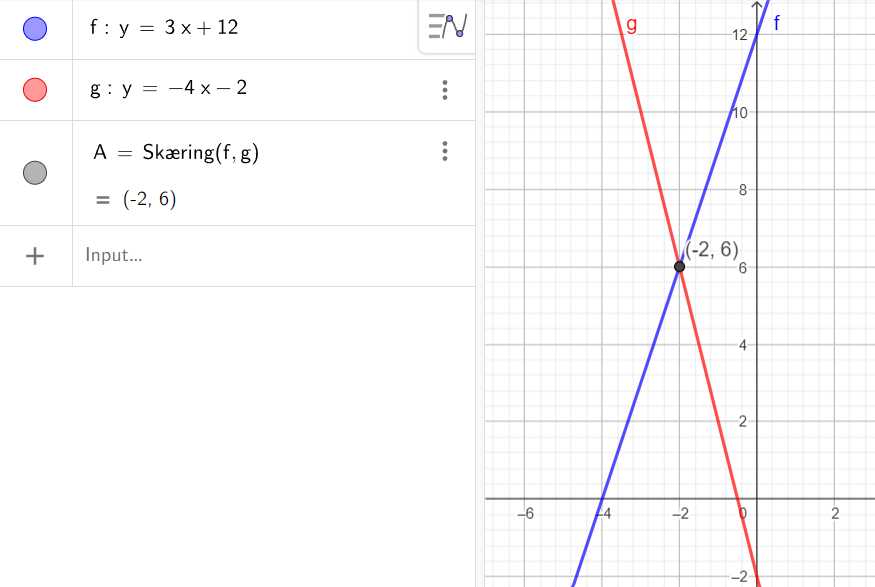
\includegraphics[width=0.8\textwidth, height=0.25\textwidth]{ans_9}
\caption{Skæringspunktet $(-2,6)$ mellem de 2 linjer $y = 3x +12$ og $y = -4x -2$}
\end{figure}

\newpage 

\textbf{Opgave 10:}

\begin{figure}[ht]
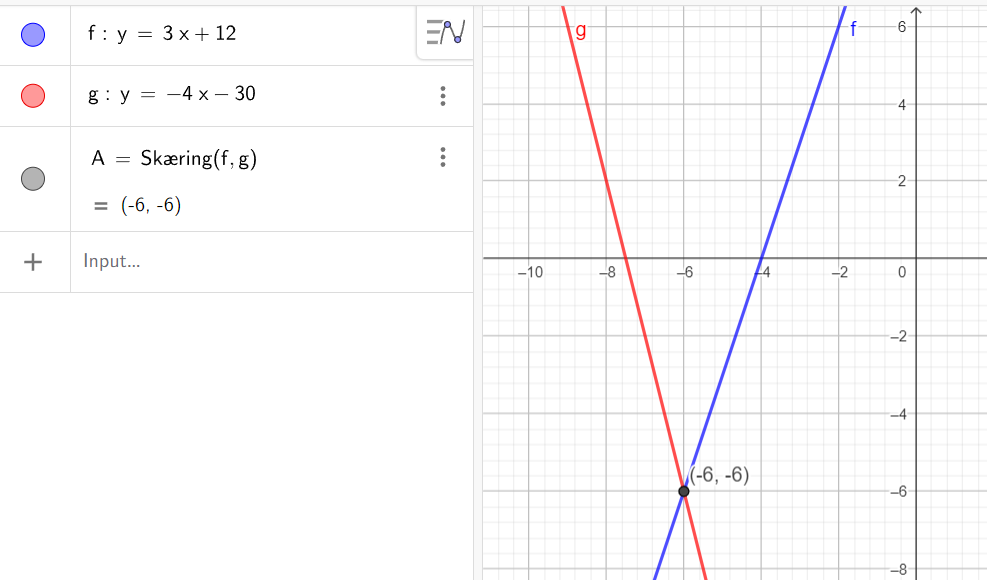
\includegraphics[width=0.8\textwidth, height=0.25\textwidth]{ans_10}
\caption{Skæringspunktet $(-6,-6)$ mellem de 2 linjer $y = 3x +12$ og $y = -4x -30$}
\end{figure}
